\chapter{Advanced Computer Graphics}
\label{chap:advanced_computer_graphics}

\begin{figure}[ht]
	\hfill
	\begin{minipage}{0.5\textwidth}
		\centering
		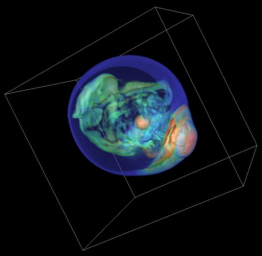
\includegraphics{VTKTextbook-104}\\
		\caption*{\texttt{Volume rendering of a supernova dataset.}}
	\end{minipage}
\end{figure}

\firstletter{C}hapter 3 introduced fundamental concepts of computer graphics.
A major topic in that chapter was how to represent and render geometry using surface primitives such as points, lines, and polygons.
In this chapter our primary focus is on volume graphics.
Compared to surface graphics, volume graphics has a greater expressive range in its ability to render inhomogeneous materials, and is a dominant technique for visualizing 3D image (volume) datasets.

We begin the chapter by describing two techniques that are important to both surface and volume graphics.
These are simulating object transparency using simple blending functions, and using texture maps to add realism without excessive computational cost.
We also describe various problems and challenges inherent to these techniques.
We then follow with a focused discussion on volume graphics, including both object-order and image-order techniques, illumination models, approaches to mixing surface and volume graphics, and methods to improve performance.
Finally, the chapter concludes with an assortment of important techniques for creating more realistic visualizations.
These techniques include stereo viewing, antialiasing, and advanced camera techniques such as motion blur, focal blur, and camera motion.

\section{Transparency and Alpha Values}
\label{sec:transparency_alpha}

Up to this point in the text we have focused on rendering opaque objects — that is, we have assumed that objects reflect, scatter, or absorb light at their surface, and no light is transmitted through to their interior. Although rendering opaque objects is certainly useful, there are many applications that can benefit from the ability to render objects that transmit light. One important
application of transparency is volume rendering, which we will explore in greater detail later in the chapter.

\section{Texture Mapping}

Texture mapping is a technique to add detail to an image without requiring modelling detail. Texture mapping can be thought of as pasting a picture to the surface of an object. The use of texture mapping requires two pieces of information: a \emph{texture map} and \emph{texture coordinates}. The texture map is the picture we paste, and the texture coordinates specify the location where the picture is pasted. More generally, texture mapping is a table lookup for color, intensity, and/or transparency that is applied to an object as it is rendered. Textures maps and coordinates are most often two-dimensional,
but three-dimensional texture maps and coordinates are supported by most new graphics hardware.

\section{Volume Rendering}
\label{sec:volume_rendering}

Until now we have concentrated on the visualization of data through the use of geometric primitives such as points, lines, and polygons.
For many applications such as architectural walk-throughs or terrain visualization, this is obviously the most efficient and effective representation for the data.
In contrast, some applications require us to visualize data that is inherently volumetric (which we refer to as 3D image or volume datasets).
For example, in biomedical imaging we may need to visualize data obtained from an MR or CT scanner, a confocal microscope, or an ultrasound study.
Weather analysis and other simulations also produce large quantities of volumetric data in three or more dimensions that require effective visualization techniques.
As a result of the popularity and usefulness of volume data over the last several decades, a broad class of rendering techniques known as volume rendering has emerged. The purpose of volume rendering is to effectively convey information within volumetric data.
\section{3D Widgets and User Interaction}
\label{sec:3dwui}
Chapter 3 provided an introduction to interaction techniques for graphics (see ``Introducing vtkRenderWindowInteractor'' on page \pageref{pg:rwi} ).
In the context of visualization, interaction is an essential featureof systems that provide methods for data exploration and query. The classes
vtkRenderWindowInteractor and vtkInteractorStyle are core constructs used in VTK to capturewindowing-system specific events in the render window, translate them into VTK events, and then take action as appropriate to that event invocation.
In Chapter 3 we saw how these classes could be used to manipulate the camera and actors to interactively produce a desired view. This functionality,
however, is relatively limited in its ability to interact with data. For example, users often wish tointeractively control the positioning of streamline starting points, control the orientation of a clipping plane, or transform an actor. While using interpreted languages (see ``Interpreted Code'' on page \pageref{pg:rwi} ) can go a long way to provide this interaction, in some situations the ability to see what you are doing when placing objects is essential. Therefore, it is apparent that a variety of user interaction techniques is required by the visualization system if it is to successfully support real-world applications.

%\printbibliography


\section{Exercises}
	